\begin{figure*}[htb]
  \centering
  \begin{subfigure}[t]{0.33\textwidth}
    \centering
    \includegraphics[width=\textwidth]{figures/profile-mot.pdf}
    \caption{Pedestrian Detection}
    \label{fig:pd-profile}
  \end{subfigure}
  \hfill
  \begin{subfigure}[t]{0.33\textwidth}
    \centering
    \includegraphics[width=\textwidth]{figures/profile-darknet.pdf}
    \caption{Augmented Reality}
    \label{fig:ar-profile}
  \end{subfigure}
  \hfill
  \begin{subfigure}[t]{0.33\textwidth}
    \centering
    \includegraphics[width=\textwidth]{figures/profile-topk.pdf}
    \caption{Top-k}
    \label{fig:tk-profile}
  \end{subfigure}
  \caption{Application profiles of three applications. Each cross point is one
    configuration $c$'s performance $(B(c), A(c))$. All figures show the Pareto
    boundary as well as the performance if only one dimension is tuned. Note the
    x-axis is in log scale.}
  \label{fig:all-profiles}
\end{figure*}

\newpage

\section{Evaluation}
\label{sec:evaluation}

In this section, we show the evaluations of \sysname{}. The results are
summarized as follows.

\begin{itemize}
\item[\autoref{sec:application-profiles}] \sysname{} generates Pareto-optimal
  profiles across multiple dimensions with precision
  (\autoref{fig:all-profiles}).
\item[\autoref{sec:online-profiling}] Our parallel and partial profiling speeds
  up offline and online profiling (\autoref{fig:parallel},
  \autoref{fig:online-tricks}).
\item[\autoref{sec:runtime-adaptation}] At runtime, \sysname{} applications
  achieve sub-second latency and nominal accuracy drop
  (\autoref{fig:all-runtime}).
\item[\autoref{sec:multi-task-alloc}] \sysname{} profiles allow different
  resource allocations, such as utility fairness (\autoref{fig:multitask}).
\end{itemize}

\subsection{Application Profiles}
\label{sec:application-profiles}

We run our offline profiling using the training dataset described
in~\autoref{tab:apps}.  \autoref{fig:all-profiles} shows the learned
profiles. In each figure, the cross dots represent the bandwidth demand and
application accuracy of one configuration. The Pareto-optimal boundary
$\mathbb{P}$ is highlighted with the blue dashed line. To understand each
dimension's impact on the degradation, we highlight configurations from tuning
only \textit{one} dimension. From these profiles, we make the following
observations:

\para{Large bandwidth variation.} For all three applications, their bandwidth
requirements have two to three orders of magnitude of difference (note the
x-axis is in log scale). For PD and AR, the most expensive configuration
transmits videos at 1080p, 30 FPS and 0 quantization; it consumes 230 mbps. In
constrast to the large bandwidth variation, there is a smaller variation in
accuracy. In PD, for example, even after the bandwidth reduced to 1 mbps (less
than 1\% of the maximum), the accuracy is still above 75\%. This allows
\sysname{} applications to operate at a high accuracy configuration even under
severe network deterioration.

\para{Multiple dimensions achieve the optimal.} Comparing dashed lines in each
profile, we see that the Pareto-optimal configurations are only achievable when
multiple knobs are in effect. Tuning only one dimension often leads to
sub-optimal performance. In Top-K, the Pareto-optimal points are mostly achieved
with tuning \texttt{N}. While \texttt{T} doesn't contribute much with this
dataset, if we use another dataset with a different distribution, the behavior
will be different.

\para{Each dimension affects differently}. Within a single profile, the
difference between tuning individual dimensions is evident. For PD, tuning
resolution (the purple line) leads to a quicker accuracy drop in comparison to
tuning the frame rate (the green line). Comparing PD and AR, the same dimension
has different impact. Tuning resolution is less harmful in AR than PD; while
tuning frame rate hurts AR more than PD. This echoes our initial observation
in~\autoref{sec:making-case-sys-approach} that application- and context-specfic
strategy doesn't generalize

\para{Quantification with precision}. The generated profiles are actionable
configurations that control the knobs with precision. In PD with our training
dataset, if the application transmits video at 1920x1080 resolution, 10FPS and
the quantizer is 20, it will consume 11.7 mbps of bandwidth, achieving roughly
90\% accuracy. This saves developers from laboriously analyzing their
application to compute manual policies.

\subsection{Profiling Efficiency and Online Profiling}
\label{sec:online-profiling}

This section focuses on the AR application as a case study. AR allows 216
different configurations: 6 resolutions, 6 frame rates and 6
quantizers. Processing a frame with YOLO~\cite{redmon2016yolo9000} on
GeForce\textregistered\space GTX 970 takes roughly 30 ms.\footnote{YOLO resizes
  an input image to a fixed neural network size. Evaluating all images (with
  different resolutions) takes a similar amount of time.} But different
configurations have different amounts of processing to do. For example, a 10FPS
video will process 1/3 of the frames in comparison to a 30FPS video. In our
experiment, to evaluate all 216 configurations, it takes 52 seconds for 1-second
worth of data. We denote such overhead as 52X. In
\autoref{sec:automatic-profiling}, we discussed techniques to improve the
profiling efficiency. We then present the evaluations as follows.

\begin{figure}
  \centering
  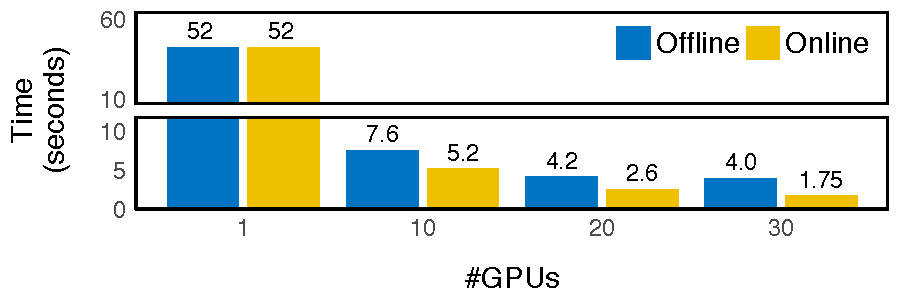
\includegraphics[width=0.9\columnwidth]{figures/parallel.pdf}
  \caption{We exploit parallelism to speed up the profiling. The y-axis shows
    the profiling time for one-second video.}
  \label{fig:parallel}
\end{figure}

\begin{figure}
  \centering
  \begin{subfigure}[t]{0.48\columnwidth}
    \centering
    \includegraphics[width=\textwidth]{figures/online1.pdf}
    \caption{Offline only}
    \label{fig:offline}
  \end{subfigure}
  \hfill
  \begin{subfigure}[t]{0.48\columnwidth}
    \centering
    \includegraphics[width=\textwidth]{figures/online2.pdf}
    \caption{Online (continuous)}
    \label{fig:online}
  \end{subfigure}
  \\
  \vspace{1.5em}
  \begin{subfigure}[t]{0.48\columnwidth}
    \includegraphics[width=\textwidth]{figures/online3.pdf}
    \caption{Online (partial)}
    \label{fig:online-partial}
  \end{subfigure}
  \hfill
  \begin{subfigure}[t]{0.48\columnwidth}
    \includegraphics[width=\textwidth]{figures/online4.pdf}
    \caption{Online (trigger)}
    \label{fig:online-trigger}
  \end{subfigure}
  \caption{The bandwidth estimation of various profiling schemes. The horizontal
    reference line is the target bandwidth (11 mbps). We omit the accuracy
    prediction since all schemes are similarly high (\textasciitilde 90\%).}
  \label{fig:online-tricks}
\end{figure}

%% Offline: 0
%% Online: 1 frame (1852.21 GPU * seconds)
%% Online (1/10)   (185.2 GPU * seconds)
%% Trigger         ( GPU * seconds)

\begin{table}[t]
  \centering
  \begin{tabular}{c c c}
    \toprule
    \specialcell{online\\ (continous)} &  \specialcell{online\\ (partial data)} & \specialcell{online\\ (partial configuration)} \\
    \midrule
    52X   & 17X              & 6X \\
    \bottomrule
  \end{tabular}
  \caption{Sampling-based profiling speeds up the profiling.}
  \label{tab:online}
\end{table}

\para{Parallelism reduces the profiling time}. Because evaluating each
individual configuration is independent of other configurations, we parallelize
the profiling task by assigning configurations to GPUs. (i) In the offline
profiling, because we do not assume a performance model among the
configurations, the assignment is random. \autoref{fig:parallel} shows that with
the increased number of GPUs, the profiling overhead reduces significantly (from
52X to 4X with 30 GPUs). (ii) The saving is further improved during the online
profiling. The processing times during the offline profiling help schedule the
assignment. With LPT assignment, the overhead is reduced to 1.75X with 30 GPUs.

\para{Partial and trigger-based online profiling.} Before we evaluate these two
schemes, we validate the \textit{concept drifts} issue with real-world data. We
use the profile trained over a video clip of the office environment. Suppose
there is 11 mbps available bandwidth, according to the profile, the application
should operate at a configuration of 1280x720 resolution, 30 FPS and a
quantization factor of 20. The test video is collected in a home environment. At
about 100 seconds, the camera points out of the window to detect objects on the
street.  Because of the scene change, the configuration fails to predict the
actual bandwidth, as illustrated in \autoref{fig:offline}.

To correct the profile, if we continuously run the profiling online and update
the strategy, the application will be able to predict the right bandwidth
demand. \autoref{fig:online} shows the bandwidth prediction when we continuously
profile with the past chunk (30 seconds of video). At time t=120s, the new
prediction matches the test data. The downside of a continuous profiling, as
discussed earlier, is the cost: 52X overhead with 1 GPU. In addition to
parallelism, two more techniques can be used for online profiling (their savings
area summarized in \autoref{tab:online}):

(i) Partial data: Instead of using all the past data, we run profiling with only
a fraction of the raw data, e.g. 1/3 of the video.  \autoref{fig:online-partial}
shows the bandwidth prediction if we only use 10 seconds of data out of the past
30 seconds. In this way, although the profile model may be less accurate (the
mis-prediction at 80-100 seconds), and there is a delay in reacting to data
change (the mis-prediction is corrected after 125 seconds), we save the online
profiling by 3X (from 52X to 17X) because of the reduction in the data that
needs to be processed.

(ii) Partial configurations: If we use the past profile as a reference and only
measure a subset of all Pareto-optimal configurations, the savings can be
substantial. A full profiling is only triggered if there is a significant
difference. \autoref{fig:online-trigger} shows the bandwidth prediction if we
evaluate 5 configurations continously and trigger a full profiling when the
bandwidth estimation is off by 1 mbps or the accuracy is off by 10\%. With our
test data, such a trigger-based profiling is enough to correct the profile.  And
the overhead is reduced to 6X because we run full profiling less often.

When we combine the parallelization and partial/trigger-based profiling, we can
further reduce the profiling overhead. For example, scheduling five GPUs running
5 configurations continuously to check for concept drifts will reduce the
overhead to almost 1X. How much resources to use will depend on the budget and
the importance of the job.

\begin{figure*}
  \begin{subfigure}{\linewidth}
    \centering
    \includegraphics[width=0.9\columnwidth]{figures/runtime-legend.pdf}
  \end{subfigure}

  \begin{subfigure}{0.3\textwidth}
    \centering
    \includegraphics[width=\textwidth]{figures/runtime-mot-verticle.pdf}
    \caption{Pedestrian Detection}
    \label{fig:pd-runtime}
  \end{subfigure}
  \hfill
  \begin{subfigure}{0.3\textwidth}
    \centering
    \includegraphics[width=\textwidth]{figures/runtime-darknet-verticle.pdf}
    \caption{Augmented Reality}
    \label{fig:ar-runtime}
  \end{subfigure}
  \hfill
  \begin{subfigure}{0.3\textwidth}
    \includegraphics[width=\textwidth]{figures/runtime-topk-verticle.pdf}
    \caption{Top-k}
    \label{fig:tk-runtime}
  \end{subfigure}
  \caption{Runtime behavior of \sysname{} applications in comparison with
    streaming over TCP/UDP.}
  \label{fig:all-runtime}
\end{figure*}

\newpage

\subsection{Runtime Adaptation}
\label{sec:runtime-adaptation}

In this section, we evaluate the runtime performance for three applications. We
first show that \sysname{} achieves low latency and high accuracy across all
three applications---demonstrating the effectiveness of our system level
approach. We then focus on AR by evaluating how manual policies and
application-specific solutions work poorly, i.e., describe the experiments for
\autoref{fig:intro}.

\para{Methodology:} We conduct our experiments on five geo-distributed machines
from Amazon EC2, spanning different AWS regions. Four act as worker nodes
(\textit{t2.micro} instances) and one acts as the aggregation server
(\textit{m4.xlarge} instance to guarantee enough bandwidth). During each
experiment, the worker node transmits test data (\autoref{tab:apps}) for about
10 mins. If the duration of the test data is less than 10 mins, we loop around.

We compare \sysname{} applications with baseline applications built with vanilla
TCP and UDP. For streaming over TCP, we use \sysname{} but disable the
adaptation. For streaming over UDP, our experiment setup is different: for video
streaming (PD and AR), we use RTSP over UDP with ffmpeg~\cite{bellard2012ffmpeg}
; for TK, we implemented a simple application protocol (packetization and custom
header) based on UDP so that the receiver can still aggregate data when loss
occurred.

Because the baselines don't adapt the configuration and $c_{max}$ is
prohibitively large---for example, raw videos consumes 230 mbps---we use a
reasonable configuration to limit the maximum rate. For PD, $c_{max}$ is
1920x1080 resolution, 10 FPS and a quantization factor of 20; it consumes about
12 mbps. For AR, $c_{max}$ is 1600x900 resolution, 30 FPS and a quantization of
20; it consumes about 14 mbps. For TK, we always truncate the windowed logs
using \texttt{head} operation with $N=9750$.

Our experiments design follows JetStream~\cite{rabkin2014aggregation}. During
the experiment, we use Linux \texttt{tc} utility with HTB scheduler~\cite{lartc,
  htb} to control the clients' outgoing bandwidth variation. Our experiments
involve four phases: (i) before time 200 seconds, there is no shaping; (ii) at
time 200 second, we start traffic shaping for 3 minutes (7.5 mbps for video
streaming and 1 mbps for TK); (iii) at time 380 second, we further decrease the
available bandwidth (5 mbps for video streaming and 0.75 mbps) for TK); (iv) at
time 440 second, all traffic shaping is removed. For UDP, HTB doesn't emulate
the packet loss or out-of-order delivery; we use \texttt{netem} and configure
the loss probability to match the delivery rate. Because different pair-wise
connections have different capacity, we impose a \textit{background} bandwidth
limit---25 mbps for PD and AR, 2.5 mbps for TK---to simplify comparisons.

The throughput figures of \autoref{fig:all-runtime} show the effect of our
traffic shaping. During the shaping, TCP and UDP make full use of the available
bandwidth; in comparison, \sysname{} is conservative. When we stop the shaping,
TCP has a ``catch-up'' phase where it's sending all the queued items as fast as
possible. \sysname{} increases the throughput gradually instead of drastically
as TCP/UDP does. This is when \sysname{} is slowly probing for more bandwidth.

The latency figures show that \sysname{} maintains a bounded latency. Note the
figures split in the middle because of the large variation in the achieved
latency. Specifically, during the traffic shaping, TCP queues items at the
sender side for up to tens or hundreds of seconds. We plot such high latency
measurements in log scale. UDP always transmits as fast as possible, leading to
a consistent low latency. \sysname{}'s latency is slightly higher than UDP but
considerable small in comparison to TCP. During the traffic shaping, \sysname{}
updates the application's degradation to avoid data queueing up. For most of the
time, we've maintained less than 500 ms latency for PD/AR, and 2.5 seconds
latency for TK. Because TK's source is triggered every second after the
\texttt{window} operation, two objects in the queue would lead to two seconds
latency. The worst case happens at the start of bandwidth drop. \sysname{}
achieves sub-second latency for PD/AR and 5 seconds latency for TK at worst
case.

The accuracy figures show that \sysname{} maintains a high accuracy throughout
the experiments. TCP without adaptation always sends data at high fidelity
(\textasciitilde 90\% for PD/AR and \textasciitilde 100\% for TK). The high
fidelity is achieved at the expense of increase latency. UDP without adaptation
suffers from packet loss, leading to a severe performance deterioration.  In
both PD and AR, the accuracy are \textasciitilde 0\% as the recovered images
contain large blocks of pixels without content details. For TK, the accuracy has
dropped to \textasciitilde 50\% during modest traffic shaping and dropped
further to \textasciitilde 25\% during the severe shaping. While \sysname{} also
sees accuracy drop during the traffic shaping, the amount is significant
smaller. We attribute this to the knowledge of the profile and a proper
configuration use during the traffic shaping.

In summary, our evaluation shows that \sysname{}'s adaptation achieves low
latency and high accuracy simultaneously.

\fixme{rewrite} Experiment data: We use AR. The manual policies are derived from
the example from JetStream~\cite{rabkin2014aggregation}. We use PD's profile as
the application-specific solution for AR. \sysname{}, Streaming over UDP and TCP
are results above. We only use the data between 200 seconds and 440 seconds,
i.e. during traffic shaping. This produces figure 1: the center is medians and
the ellipses are standard deviations.

\subsection{Resource Allocation and Fairness}
\label{sec:multi-task-alloc}

We evaluate resource allocations with two applications. In this way, the results
cover the case of a single application, and can be generalized to more
applications.

We choose PD and AR as the example applications. The setup is the same as
before; both applications share the same client and server, therefore, they
share the same bottleneck link. The experiment starts with sufficient
bandwidth. At 60 seconds, we start traffic shaping to limit the total bandwidth
at 6 mbps. When we allocate resource equally between two applications
(\autoref{fig:eq-bw}), each application will get 3 mbps. Under this condition,
PD runs with a higher accuracy (\textasciitilde 85\%) while AR only achieves
\textasciitilde 77\%. In contrast, \sysname{} also supports utility fairness: it
chooses configurations that maximize the minimal accuracy. In this experiment,
PD receives 2 mbps and AR receives 4 mbps; and both achieve \textasciitilde 80\%
accuracy (\autoref{fig:eq-acc}).

\begin{figure}
  \begin{subfigure}[t]{0.9\columnwidth}
    \centering
    \includegraphics[width=\textwidth]{figures/multitask-legend.pdf}
  \end{subfigure}
  \\
  \vspace{1em}
  \begin{subfigure}[t]{0.49\columnwidth}
    \centering
    \includegraphics[width=\textwidth]{figures/multitask-eq-bw.pdf}
    \caption{Resource Fairness}
    \label{fig:eq-bw}
  \end{subfigure}
  \hfill
  \begin{subfigure}[t]{0.49\columnwidth}
    \centering
    \includegraphics[width=\textwidth]{figures/multitask-eq-acc.pdf}
    \caption{Utility Fairness}
    \label{fig:eq-acc}
  \end{subfigure}
  \caption{Comparison between different schemes of resource allocations:
    resource fairness and utility fairness.}
  \label{fig:multitask}
\end{figure}

%%% Local Variables:
%%% mode: latex
%%% TeX-master: "sosp17"
%%% End:
